\chapter{Bundling proteins' dynamics and effects on actin binding proteins}\label{ch:abp-bundle}

\section[Abstract]{Abstract\footnotemark}

Collaboration with John, Jenna, Katie, and Cristian in the Kovar lab to understand the role that different bundlers play when it comes to regulating other ABPs.

Bundling proteins found in a wide variety of actin networks

Bind along actin filaments and can dictate the filament architecture

How do bundling proteins effect localization and dynamics of other ABPs?

\footnotetext{Citations for chapter: [1] Jonathan D. Winkelman, Cristian Suarez, Glen M. Hocky, Alyssa J. Harker, Alisha N. Morganthaler, Jenna R. Christensen, Gregory A. Voth, James R. Bartles, and David R. Kovar Fascin- and $\alpha$-Actinin-Bundled Networks Contain Intrinsic Structural Features that Drive Protein Sorting. \textit{Current Biology}, 26{20}:2697-2706, October 2016. [2] Jenna R. Christensen, Kaitlin E. Homa, Alisha N. Morganthaler, Cristian Suarez, Alyssa J. Harker, Meghan O'Connell, and David R. Kovar. \textit{In preparation.}}

\section{Introduction}\label{ch03-introduction}

Many bundling proteins bind cooperatively to sides of filaments, 
meaning that once one bundling protein binds, another of the same 
protein is more likely to bind in the next available binding site 
than random chance \citep{winkelman_fascin-_2016}. This positive 
feedback mechanism facilitates bundle formation as many bundlers can
bind along the length of the two filaments. Additionally, the 
cooperatively allows continuous domains of the bundlers to form.

Bundling proteins have a large effect on the different architectures of 
F-actin networks. Depending on their dynamics and size they can dictate 
the orientation and spacing of the filaments in the network as well as 
the stability of the bundles. For example, filopodia and lamellipodia 
are not separated in space but have very distinct filament orientations. Lamellipodia filaments are branched by Arp2/3 complex and kept short by
capping protein. Fimbrin localizes to the lamellipodia and crosslinks 
these filaments into a dense meshwork. In contrast, filopodia contain long, straight F-actin bundled primarily by fascin.  It is unclear the importance
of each bundling protein is for initiating and maintaining each network
to which it localizes. 

Another difference in network architecture is in stress fibers compared to filopodia. Filaments are narrowly spaced within filopodia, while stress 
fibers have wider spacing due to the main bundling proteins fascin and 
$\alpha$-actinin, respectively. Fascin is a small globular bundling protein compared to the homodimer $\alpha$-actinin. We were interested if the intrinsic properties of the bundling proteins themselves could lead to different 
sorting between bundling proteins and therefore could lead to different
architectures within cells. 

Recently we found that two bundling proteins, fimbrin and $\alpha$-actinin, can compete only in the presence of an additional side binding protein, tropomyosin in S. Pombe \citep{christensen_competition_2017}. Tropomyosin is a coiled-coil protein that binds along the sides of F-actin and is known to stabilize F-actin as well as effect other ABP binding. The competition between fimbrin and alpha-actinin in S. Pombe is interesting since fission yeast alpha-actinin is an especially poor bundling protein with high dynamics. Additionally in cells, we see that tropomyosin and alpha-actinin localize to the cytokinetic ring where fimbrin mainly localizes to endocytic actin patches. That tropomyosin can bolster alpha-actinin’s bundling properties and competition against fimbrin could be important for the different network architectures and how different ABPs are sorted. 

\section{Results}

\subsection{Fascin and \texorpdfstring{$\alpha$}{a}-actinin sort to distinct domains}

\begin{figure}
\centering
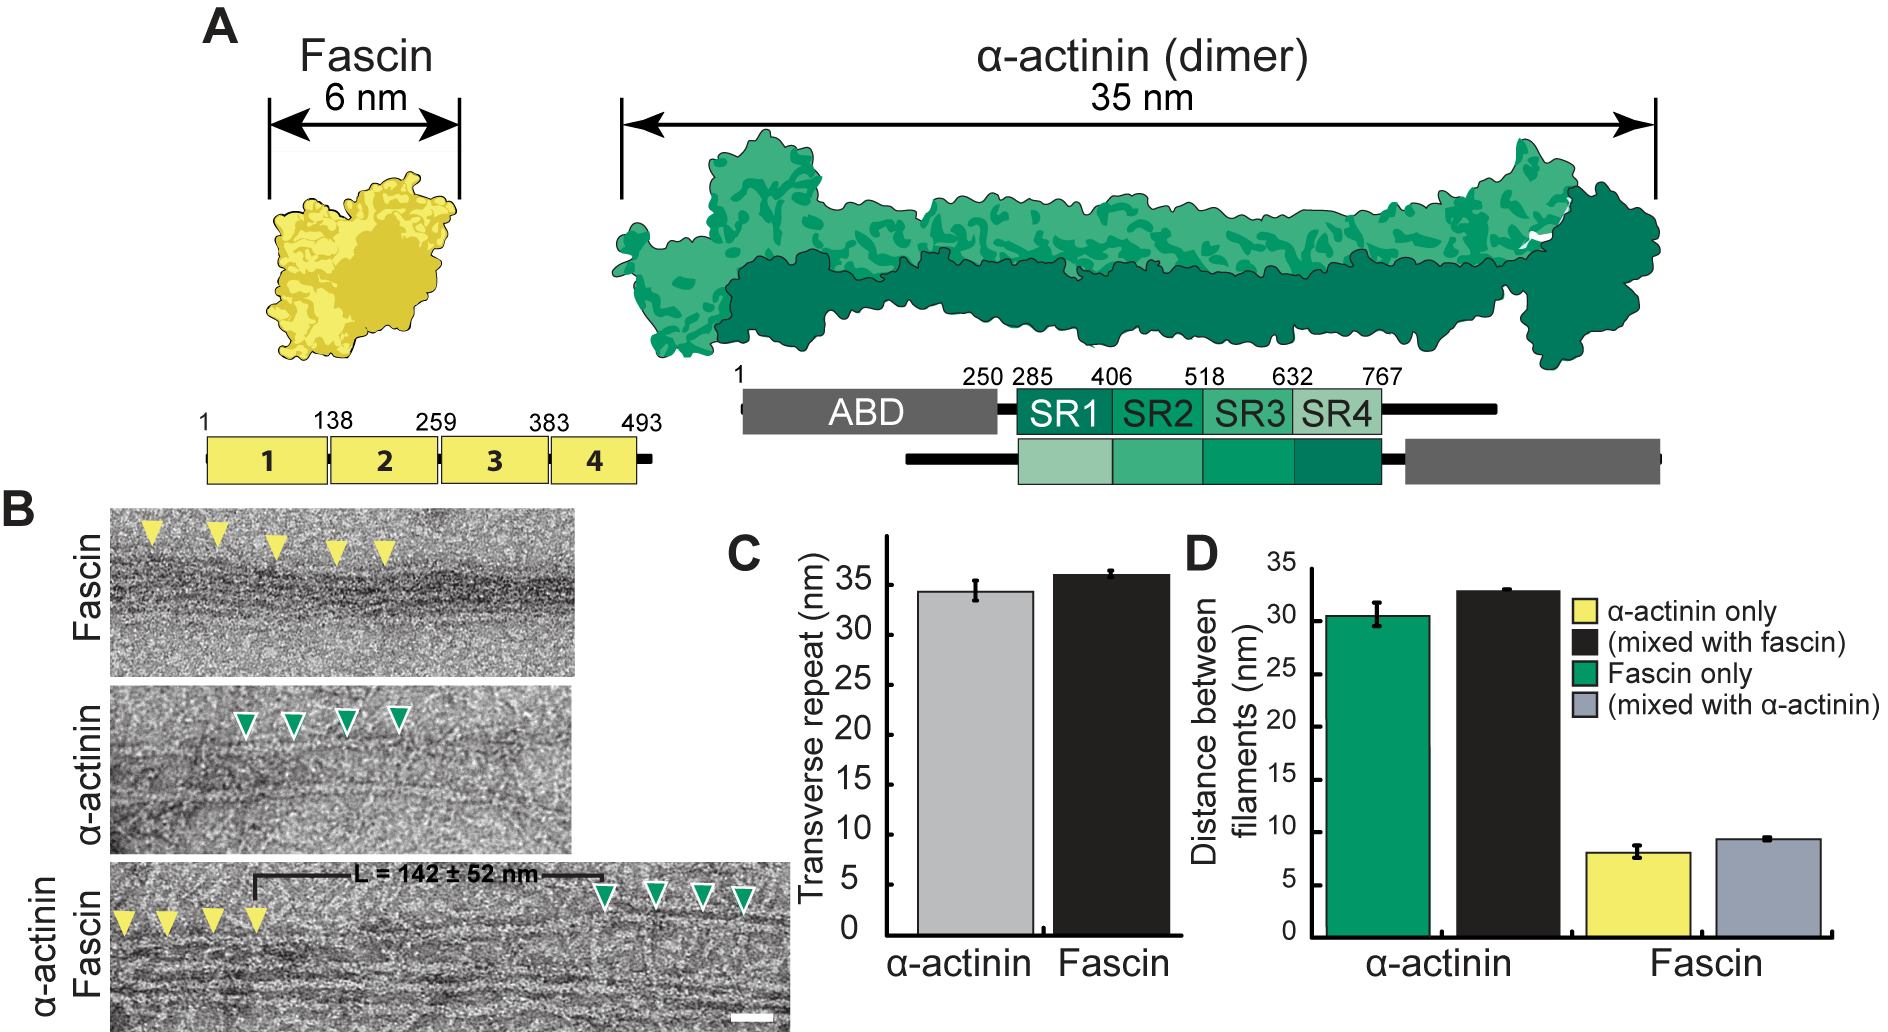
\includegraphics[width=14cm]{img/ch03/Thesis_EM_fig.png}
\caption[Ena constructs have the predicted oligomerization state.]{\textbf{Ena constructs have the predicted oligomerization state.} (A) Structural fold (top) and domain organizations (bottom) showing the four $\beta$-trefoil domains of fascin (PDB 3P53; \citep{jansen_mechanism_2011}) (left) and an $\alpha$-actinin dimer (PDB 1SJJ; {liu a 3D}) (right). ABD, Actin-binding domain; SR, spectrin repeat. (F–H) Electron microscopy (EM) of F-actin bundles negatively stained with uranyl acetate, which were formed from 1.5 $\mu$M actin.(F) Micrographs of bundles with 1 $\mu$M fascin (top), 800 nM $\alpha$-actinin (middle) or both (1 $\mu$M $\alpha$-actinin 0.25 $\mu$M fascin (bottom). Yellow and green arrowheads indicate fascin and $\alpha$-actinin molecules. L is length of transition zone. Scale bar = 30 nm. (G) Distance of transverse repeat in fascin and $\alpha$-actinin bundles. Error bars indicate SEM; $n\geq10$ bundles. (H) Distance between filaments in a fascin and $\alpha$-actinin bundles. Error bars indicate SEM; $n\geq8$ bundles. Figure adapted from \citep{winkelman_fascin-_2016}. \textbf{EM in collaboration with Cristian Suarez.}}
\label{fig:em_fascin_aact}
\end{figure}

\subsection{Tropomyosin effects \texorpdfstring{$\alpha$}{a}-actinin dynamics}


